\chapter{Estudio de alternativas}

\section{Análisis de Alternativas actualmente disponibles en el mercado}

En la actualidad, en la extensión de la investigación, existen productos comerciales y proyectos privados que se asemejan a las características ofrecidas por el proyecto, son en su mayoría de índole privatizada especialmente en el campo de la medicina, donde solo se hace mención a sus resultados, sin embargo, ninguna resalta por su accesibilidad gratuita, distinguiendo el proyecto del factor común. Siendo las aplicaciones y programas desarrollados con un enfoque principal en entretenimiento, como es el caso de videojuegos y medicina, en analizadores médicos y programas de rehabilitación.\\

\subsubsection{Analizadores Médicos}

En la rama de la medicina, la información es más privatizada o proporciona un menor alcance al publico, solo reporta resultados y posibles cambios y amplitudes afirmando la falta de pruebas para dar mayor información, por lo que profundizar en ello no otorgara profundidad al proyecto, no obstante, se ha encontrado que se utiliza la tecnología planeada para controlar la pose del usuario, ya sea en pruebas médicas para hallar anormalidades físicas en la posición del cuerpo al realizar diversas actividades y en entrenamiento físico para mantener una posición estable y evitar dañarse a uno mismo.

\subsection{Entretenimiento}

Cuando se referencia a un sistema de estimación de pose del cuerpo, se nombran varios títulos de videojuegos de baile, siendo las primeras y más importantes sagas, las desarrolladas por Ubisoft como Just Dance o Dance Experience, enfocadas en realizar coreografías pre-diseñadas para canciones populares en la época del lanzamiento de sus entregas; a pesar de que en Just Dance han existido niveles con temática de artes marciales, estas no contaban con la intención de ser un entrenamiento educativo, sino un baile con el propósito de entretener utilizando movimientos basados del arte marcial.  \\
\\
Además de las mencionadas, existe otro género en los videojuegos enfocado al entrenamiento físico, como Shape Up de Ubisoft y Wii Fit de Nintendo, estas enfocadas más a un entrenamiento físico casual como es el caso de Shape Up, donde se incentiva al jugador a realizar ejercicios anaeróbicos de alta intensidad como son flexiones, abdominales o sentadillas y Wii Fit enfocado a rutinas de Yoga, equilibrio y aeróbicos; demostrando las diferentes aplicaciones y posibilidades de desarrollo y resultados. \\

\subsubsection{Just Dance}

Just dance es una serie de sistemas interactivos con Body Tracking, es un producto pionero en el tema desarrollado por Ubisoft París que debuto en octubre del 2010. La serie de Just Dance cuenta con un total de 30 títulos con un amplio rango de categorías de edades para llegar a la audiencia, es ya una serie que libera un nuevo titulo al menos una vez al año, demostrando ser un éxito comercial. Gran parte de la inspiración del proyecto actual es este sistema interactivo, que emplea al máximo el controlador Kinect y el Body Tracking con comandos de voz para ofrecer un uso casual y entretenido, sin embargo, la carencia del equipo y la frustración de no ser capaces de aprovecharlo, se desvían en cambio a la posibilidad de crear una alternativa, el cual se espera que con el equipamiento provisto para el proyecto, carente de una cámara de profundidad (elemento sobresaliente en el controlador Kinect), permita el desarrollo adecuado de las características de Body Tracking.


\section{Análisis de Alternativas En Herramientas Disponibles Para el Desarrollo}

\subsection{Trajes con sensores de movimiento}

La industria actual de cine, sistemas interactivos, deportes e incluso la medicina cuentan con una inversión que llega a niveles millonarios en recrear animaciones del cuerpo humano, empleando las herramientas externas que faciliten la lectura de movimiento, su uso es bastante extendido y llega a crear obras de gran calidad, sin embargo, en su mayoría esta tecnología no esta disponible para el publico en general debido a su elevado costo, y ya que no es un campo prioritario de investigación en la Universidad Privada Boliviana, por tanto, esta alternativa queda descartada.
\\
Los trajes cuentan con 19 sensores distribuidos alrededor del cuerpo y recogen movimientos de un actor para transmitirlos en tiempo real. Una de sus ventajas es la reducción de costos en las producciones para motion capture, además de no requerir un set de estudio demasiado restrictivo para su implementación. Existen además, varios modelos del traje proporcionados por empresas como Xsens, Holosuit, Teslasuit y otros.

\begin{figure}[t!]
	\centering
	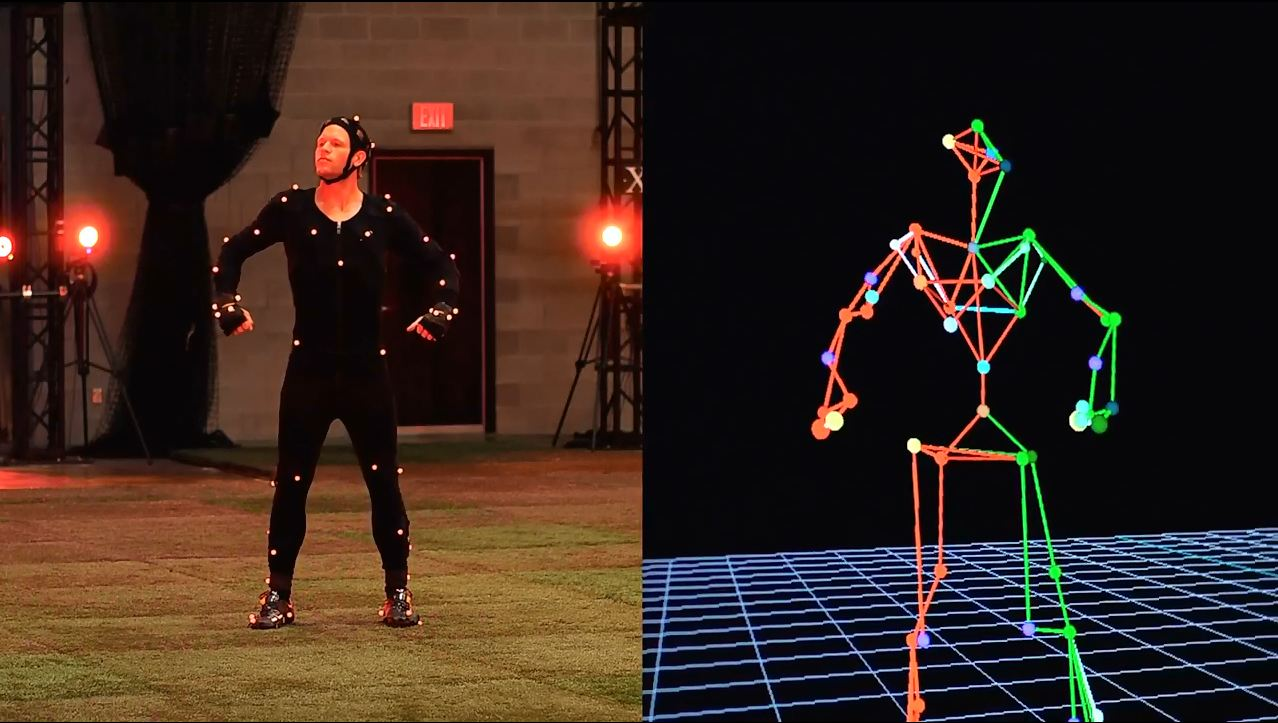
\includegraphics[width=9cm,height=4cm,]{./Images/trajesensor.jpg}
	\caption{Traje con Sensores de Movimiento}
	\label{trajesensores}
\end{figure}

\subsubsection{Creación de Software propio para Body Tracking}

Uno de los objetivos implícitos del desarrollo de este proyecto es el siguiente "El objetivo no es volver a crear la rueda, sino, crear algo nuevo utilizando esa rueda", palabras del supervisor del proyecto, por tanto, a pesar de ser un posible acercamiento a la solución, queda completamente descartada.

\subsection{TensorFlow}

\href{https://www.tensorflow.org/lite/models/pose_estimation/overview}{Tensorflow}
es una herramienta open source para machine learning provista de soporte por Microsoft, la comunidad la ha empleado extensamente en proyectos y estudios de múltiples campos de la inteligencia artificial,  de Body Tracking con el uso de PoseNet, derivado de TensorFlow, cuenta con soporte y una documentación clara, siendo además sus requisitos recomendados para su uso relativamente bajos. 
\\
Tensorflow se basa en redes neuronales para deep learning, es una herramienta interfaz que implementa algoritmos para machine learning, puede ser ejecutada con una variedad de sistemas, desde celulares hasta tablets, e incluso sistemas a gran escala. Tiene un amplio rango de algoritmos de entrenamiento, incluyendo entrenamiento e modelos de inferencia para deep neural network models e investiga ramas de múltiples ramas, incluyendo recolección de información, proceso de entendimiento de un lenguaje natural, geografía, descubrimiento de drogas, ciencias Computacionales y otros.  \cite{abadi2016tensorflow}

\subsection{Posenet}

Posenet es una herramienta desarrollado por Google Creative Lab basada en Tensorflow que permiten demostrar una estimación a tiempo real de estimación de poses (Body Tracking) en tiempo real. Esta herramienta puede ser empleada tanto para una persona a la vez como para varias personas a la vez dependiendo del algoritmo que se emplee, la diferencia es en la velocidad y simpleza en su función \cite{kendall2015posenet}.
\\
Debido a que el proyecto será para un uso singular, se mencionara su posibilidad a través del algoritmo de Body Tracking para una persona.

Emplea una imagen RGB que alimenta a la red neuronal y emplean un decodificador de poses, designando valores de confianza, posiciona puntos clave y valores de confianza para los puntos clave para el aprendizaje de la red neuronal en la lectura de imágenes con las cuales aprendió a estimar las posiciones en tiempo real\cite{oved2018real}.
\\
En cuanto los términos previos, son propios de PoseNet, por tanto se los debe explicar y mostrar visualmente para su entendimiento, los cuales se denotan en la figura \ref{exampleposenet}:

\begin{itemize}
	\item Pose: Retorna un objeto que contiene una lista de puntos clave y valores de confidencia para cada persona detectada.
	\item Valor de confidencia de pose: Determina la confianza que tiene la estimación de la pose,en un rango de 0 a 1 y puede ser usado en caso que las partes del cuerpo bloqueadas por el cuerpo mismo o elementos externos represente un obstáculo para su lectura exacta.
	\item Punto Clave: Son literalmente un grupo de puntos, es la parte que se estima del cuerpo humano para formar el esqueleto, como se observa claramente en la figura \ref{open2}. En la base de datos de modelo COCO, existen 17 puntos de lectura.
	\item Valor de Confianza de un punto clave: Determina en un rango de 0 al 1 la confianza que se tiene de la precisión del punto determinado, bajo el mismo concepto de la pose, en caso que existan obstáculos.
	\item La posición del punto clave: Las coordenadas (x,y) de la imagen en las que se encuentran los puntos claves.
\end{itemize}

\begin{figure}[ht]
	\centering
	\begin{subfigure}{.5\textwidth}
		\centering
		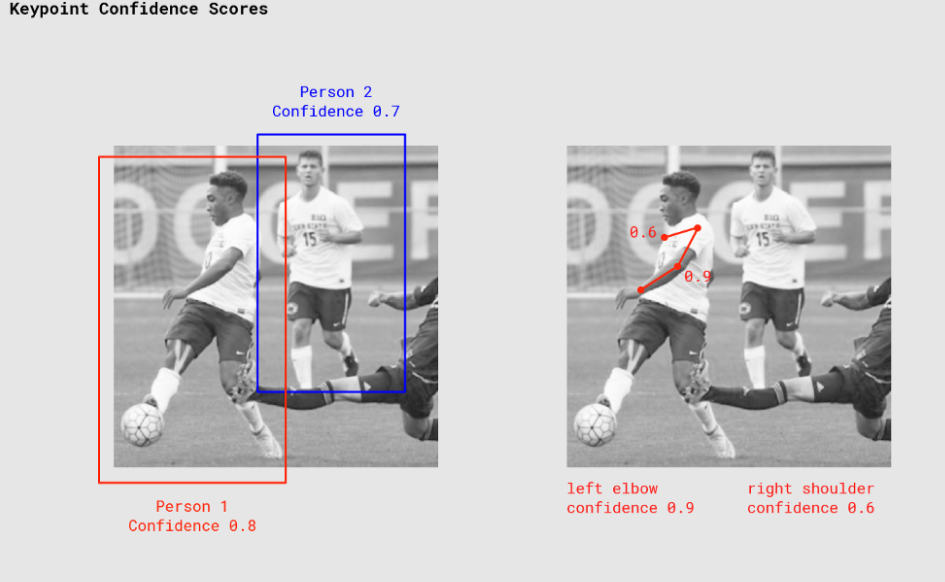
\includegraphics[width=7cm,height=5cm,]{./Images/posenetcocoexample.png}
		\caption{Ejemplo a}
		\label{posenet1}
	\end{subfigure}%
	\begin{subfigure}{.5\textwidth}
		\centering
		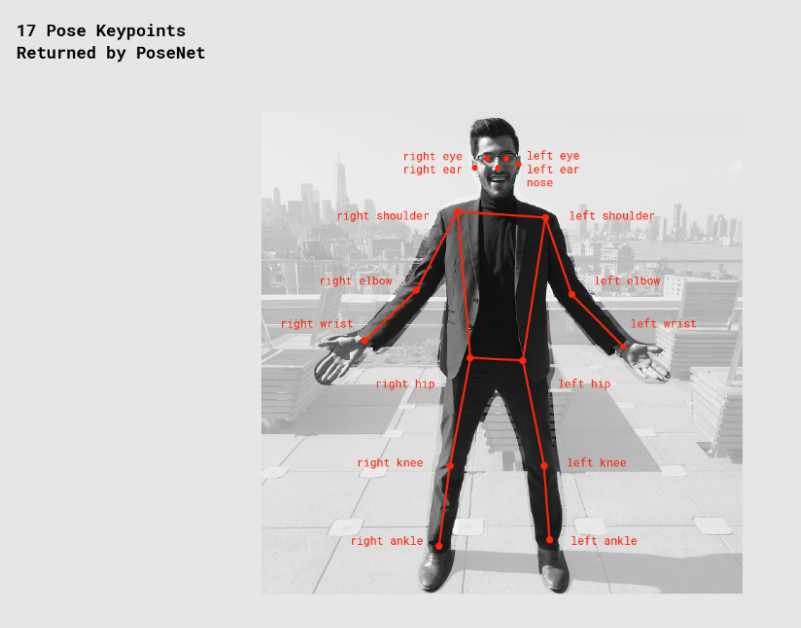
\includegraphics[width=7cm,height=5cm]{./Images/posenetexample2.png}
		\caption{Ejemplo b}
		\label{posenet2}
	\end{subfigure}
	\caption{Ejemplos de Datos en la Base de Datos COCO para la estimación de pose}
	\label{exampleposenet}
\end{figure}



Si bien esta es una herramienta con soporte constante por parte de Google y una documentación clara y amplia, la herramienta requiere de características altas por parte de los equipos empleados para usarlo, su instalación y uso no es nada sencillo y es imposible cubrir todos sus requisitos en la medida de lo posible con el corto tiempo dado por la materia, concluyendo que se requerirá de buscar otras opciones para el proyecto.

\subsection{Wrnch}

\href(https://wrnch.ai/){Wrnch} es una herramienta de calidad para el desarrollo de aplicaciones con Body Tracking, posee un gran potencial para el desarrollo del proyecto, contando con el esqueleto que se forma al seguir los movimientos de la persona, además cuenta con una opción de multiples cámaras en distintos angulos, capaz de seguir el movimiento de los dedos al mismo tiempo que el cuerpo completo casi en tiempo real. Como debilidad, la dependencia del Hardware y sus elevados requisitos para emplear al máximo esta herramienta con el equipamiento disponible, limitó sus posibilidades y uso en el proyecto.

\subsection{OpenPose}

\href{https://github.com/CMU-Perceptual-Computing-Lab/openpose}{OpenPose} es una herramienta open source desarrollada y mantenido principalmente por Gines Hidalgo, junto a su equipo de 6 personas y el apoyo de CMW Panoptic Studio Dataset. Es una herramienta principalmente programada en C++, empleando Cuda, Cmake y Shell, parte de ello para su instalación por parte de terceros que deseen desarrollar Software a partir de esta herramienta. Incluye APIs para desarrollo en Python y C++, posee un plugin para Unity desarrollado en el 2018, que a pesar de estar desactualizado, posee los mínimos requerimientos necesarios para el desarrollo del proyecto. 
Es una herramienta similar a PoseNet en cuanto a los requerimientos del proyecto, es constantemente actualizado y permite incluso el reconocimiento de puntos clave del rostro y las manos, que si bien, merece ser mencionado, no se empleara a lo largo del proyecto.

Esta es la herramienta seleccionada para el desarrollo del proyecto, por tanto, fue previamente explicado y mencionado en el Marco Teórico, para más información, favor de revisarlo nuevamente.



\subsection{DeepMotion}
\href{https://deepmotion.com/3d-body-tracking}{DeepMotion} es una herramienta de body tracking proporcionada por la compañía DeepMotion, la cual, empleando machine learning y computer vision, proveen de una solución para crear animaciones de modelos 3D con recursos mínimos en requerimientos de Hardware y experiencia requerida. Si bien, esta herramienta es rápidamente descartada debido a su alto coste y la lentitud de respuesta por parte del equipo en proporcionar el conocimiento para su adquisición, el soporte que se espera es amplio.

\subsection{Unity y Kinect}

El Kinect SDK provee a los desarrolladores de herramientas para el reconocimiento de voz empleando el uso de los sensores del dispositivo Kinect con el que funciona, además de una lectura de profundidad e infrarrojo para facilitar la motion capture. Al emplear este recurso y utilizar Unity para poder desarrollar tanto los modelos necesarios para el proyecto como la interfaz de la aplicación, se podría llegar a desarrollar el proyecto sin contratiempos e incluso con más funciones.

Sin embargo, hoy en día, el dispositivo Kinect fue descontinuado y las consolas a las que se conectan ya no incluyen el adaptador para el dispositivo. Además, se recuerda que la falta del Kinect y la búsqueda de una solución alternativa a su uso obligan a rechazar la consideración de emplear esta posible solución.










